\textbf{Цель работы:} Получние навыков разработки алгоритмов решения краевой задачи при реализации моделей, построенных на ОДУ второго порядка.

\section{ИСХОДНЫЕ ДАННЫЕ}

\subsection{Данные для тестирования}

\begin{equation*}
    \begin{matrix}
        K_0 = 0.4 \\
        K_n = 0.1 \\
        \alpha_0 = 0.05 \\
        \alpha_n = 0.001 \\
        l = 10 \\
        T_0 = 300 \\
        R = 0.5 \\
        F_0 = 50 \\
    \end{matrix}
\end{equation*}

\subsection{Уравнение для функции $T(x)$}

\begin{equation}\label{eq:t(x)}
    \frac{d}{dx} \bigg( k(x) \frac{dT}{dx} \bigg) - \frac{2}{R} \alpha(x)T +
    \frac{2T_0}{R} \alpha(x) = 0
\end{equation}

\subsection{Краевые условия}

\begin{equation*}
    \begin{cases}
        x = 0, -k(0) \frac{dT}{dx} = F_0, \\
        x = l, -k(l) \frac{dT}{dx} = \alpha_N \big( T(l) - T_0 \big)
    \end{cases}
\end{equation*}

Функция $k(x)$ представлена на формуле \ref{eq:k}

\begin{equation}\label{eq:k}
    k(x) = \frac{a}{x - b}
\end{equation}

, где

\begin{equation*}
    a = -K_0 b = \frac{K_0 K_n l}{K_0 - K_n}
\end{equation*}

\begin{equation*}
    b = \frac{K_N l}{K_N - K_0}
\end{equation*}

Функция $\alpha(x)$ представлена на формуле \ref{eq:alpha}

\begin{equation}\label{eq:alpha}
    \alpha(x) = \frac{c}{x- d}
\end{equation}

, где

\begin{equation*}
    c = -\alpha_0d = \frac{\alpha_0 \alpha_N l}{\alpha_0 - \alpha_N}
\end{equation*}

\begin{equation*}
    d = \frac{\alpha_n l}{\alpha_n - \alpha_0}
\end{equation*}

\subsection{Разностная схема}

\begin{equation}\label{eq:main}
    A_n y_{n+1} - B_n y_n + C_n y_{n-1} = -D_n, 1 \le n \le N-1
\end{equation}

\begin{equation}\label{eq:start_left}
    K_0 y_0 + M_0 y_1 = P_0
\end{equation}

\begin{equation}\label{eq:start_right}
    K_n y_n + M_n u_{n-1} = P_n
\end{equation}

\begin{equation*}
    A_n = \frac{x_{n+\frac{1}{2}}}{h},\ C_n = \frac{x_{n-\frac{1}{2}}}{h},
    \ B_n = A_n + C_n + p_n h,\ D_n = f_nh
\end{equation*}

Метод трапеций

\begin{equation*}
    x_{n \pm \frac{1}{2}} = \frac{2 k_n k_{n\pm1}}{k_n + k_{n\pm1}}
\end{equation*}

\subsection{Краевые условия}

\begin{equation*}
    F = -k(x)\frac{dT}{dx}
\end{equation*}

\begin{equation*}
    p(x) = \frac{2}{R} \alpha(x)
\end{equation*}

\begin{equation*}
    f(x) = \frac{2T_0}{R} \alpha(x)
\end{equation*}

\begin{equation*}
    p_n = p(x_n), f_n = f(x_n)
\end{equation*}

Разностные аналоги кравевых условий при $x = 0$

\begin{equation}\label{eq:left}
    y_0 \cdot \bigg( x_{\frac{1}{2}} + \frac{h^2}{8} p_{\frac{1}{2}} +
    \frac{h^2}{4}p_0 \bigg) - y_1 \cdot \bigg( x_{\frac{1}{2}} - \frac{h^2}{8}
    p_{\frac{1}{2}} \bigg) = \bigg( hF_0 + \frac{h^2}{4} \big(f_\frac{1}{2}+
    f_0 \big) \bigg)
\end{equation}

Для $p_\frac{1}{2}$ и $f_\frac{1}{2}$ можно принять простую аппроксимацию

\begin{equation*}
    p_\frac{1}{2} = \frac{p_0 + p_1}{2}
\end{equation*}

\begin{equation*}
    f_\frac{1}{2} = \frac{f_0 + f_1}{2}
\end{equation*}

Разностные аналоги кравевых условий при $x = l$. Проинтегрируем \ref{eq:t(x)} на отрезке $\big[ x_n-\frac{1}{2}; x_n \big]$

\begin{equation*}
    -\int_{X_{n-\frac{1}{2}}}^{X_n} \frac{dF}{dx} dx -
    \int_{X_{n-\frac{1}{2}}}^{X_n} p(x)T dx +
    \int_{X_{n-\frac{1}{2}}}^{X_n} f(x) dx = 0
\end{equation*}

Второй и третий интегралы вычислим методом трапеций

\begin{equation*}
    F_{n-\frac{1}{2}} - F_n -
    \frac{p_{n-\frac{1}{2}}y_{n-\frac{1}{2}} + p_ny_n}{4} h +
    \frac{f_{n-\frac{1}{2}} + f_n}{4} h = 0
\end{equation*}

Подставим в полученное уравнение

\begin{equation*}
    F_{n-\frac{1}{2}} = x_{n-\frac{1}{2}} \frac{y_{n-1} - y_n}{h}
\end{equation*}

\begin{equation*}
    F_n = \alpha_(y_n-T_0)
\end{equation*}

\begin{equation*}
    y_{n-\frac{1}{2}} = \frac{y_n + Y_{n-1}}{2}
\end{equation*}

Получим

\begin{equation*}
    \frac{x_{n-\frac{1}{2}} y_{n-1}}{h} -
    \frac{x_{n-\frac{1}{2}} y_{n}}{h} -
    \alpha_ny_n +
    \alpha_nT_0 -
    \frac{p_{n-\frac{1}{2}} y_{n-1}}{8}h -
    \frac{p_{n-\frac{1}{2}} y_{n}}{8}h -
    \frac{p_{n}y_{n}}{4}h +
    \frac{f_{n-\frac{1}{2}} + f_n}{4}h = 0
\end{equation*}

\begin{equation}\label{eq:right}
    y_n \cdot \bigg( -\frac{x_{n-\frac{1}{2}}}{h} - \alpha_n -
    \frac{p_n}{4}h - \frac{p_{n-\frac{1}{2}}}{8} h \bigg) +
    y_{n-1} \cdot \bigg( \frac{x_{n-\frac{1}{2}}}{h} -
    \frac{p_{n-\frac{1}{2}}}{8} h \bigg) = - \bigg(
    \alpha_nT_0 + \frac{f_{n-\frac{1}{2}} + f_n}{4} h \bigg)
\end{equation}

С помощью формул \ref{eq:start_left} и \ref{eq:left} получаем коэффициенты
$K_0$, $M_0$ и $P_0$, а с помощью \ref{eq:start_right} и \ref{eq:right} получаем
$K_n$, $M_n$ и $P_n$.

\subsection{Метод прогонки}

Для решения системы из \ref{eq:main}, \ref{eq:start_left} и \ref{eq:start_right}
используется метод прогонки, который состоит из двух этапов: прямой ход и
обратный ход.

\textbf{Прямой ход}

Для коэффициентов $\varepsilon$ и $\eta$ нужны начальные значения
(формулы \ref{eq:first_eps} и \ref{eq:first_eta}).

\begin{equation}\label{eq:first_eps}
    \varepsilon_1 = -\frac{M_0}{K_0}
\end{equation}

\begin{equation}\label{eq:first_eta}
    \eta_1 = \frac{P_0}{K_0}
\end{equation}

Затем вычисляются остальные элементы массива прогоночных коэффициентов
(формула \ref{eq:front_move}).

\begin{equation}\label{eq:front_move}
    y_n =
    \underbrace{\frac{C_n}{B_n - A_n \varepsilon_n}}_{\varepsilon_{n+1}} y_{n+1} +
    \underbrace{\frac{D_n + A_n \eta_n}{B_n - A_n \varepsilon_n}}_{\eta_{n+1}}
\end{equation}

\textbf{Обратный ход}

По формуле \ref{eq:last_y} находим начальное значение $y_n$.

\begin{equation}\label{eq:last_y}
    y_n = \frac{P_n - M_n \eta_n}{K_n + M_n \varepsilon_n}
\end{equation}

Остальные значения находятся по формуле \ref{eq:back_move}.

\begin{equation}\label{eq:back_move}
    y_n = \varepsilon_{n+1} y_{n+1} + \eta_{n+1}
\end{equation}

Полученный массив $y$ будет искомый массив $T(x)$.

\section{ЛИСТИНГИ}

\begin{lstlisting}[caption=Расчет начальных коэффициентов]
Mathematics::Mathematics(
    const double k0,
    const double kn,
    const double a0,
    const double an,
    const double F0
    const bool ax3
)
    : _multiAlpha(ax3 ? 3.0 : 1.0 ),
    _k0(k0), _kn(kn), _alpha0(a0), _alphaN(an), _F0(F0),
    _a((_k0 * _kn * _l) / (_k0 - _kn)),
    _b((_kn * _l) / (_kn - _k0)),
    _c((_alpha0 * _alphaN * _l) / (_alpha0 - _alphaN)),
    _d((_alphaN * _l) / (_alphaN - _alpha0))
{
    double x1_2 = (2 * k(0) * k(_h)) / (k(0) + k(_h));
    double p0 = p(0);
    double p1_2 = (p0 + p(_h)) / 2.0;
    double f0 = f(0);
    double f1_2 = (f0 + f(_h)) / 2.0;

    _K0 = x1_2 + (_h * _h / 8.0) * p1_2 + (_h * _h / 4.0) * p0;
    _M0 = -x1_2 + (_h * _h / 8.0) * p1_2;
    _P0 = _h * _F0 + (_h * _h / 4.0) * (f1_2 + f0);

    double xN1_2 = (2 * k(_l) * k(_l - _h)) / (k(_l) + k(_l - _h));
    double alphaN = alpha(_l);
    double pN = p(_l);
    double pN1_2 = (pN + p(_l - _h)) / 2.0;
    double fN = f(_l);
    double fN1_2 = (fN + f(_l - _h)) / 2.0;

    _KN = -(xN1_2 / _h) - alphaN - (pN / 4.0) * _h - (pN1_2 / 8.0) * _h;
    _MN = (xN1_2 / _h) - (pN1_2 / 8.0 * _h);
    _PN = -alphaN * _T0 - ((fN1_2 + fN) / 4.0) * _h;

    findCoeff();
    findResult();
}
\end{lstlisting}

\begin{lstlisting}[caption=Функции $k(x)$ $\alpha(x)$ $p(x)$ и $f(x)$]
double Mathematics::k(const double x)
{
    return _a / (x - _b);
}

double Mathematics::alpha(const double x)
{
    return _multiAlpha * (_c / (x - _d));
}

double Mathematics::p(const double x)
{
    return (2 * alpha(x)) / _R;
}

double Mathematics::f(const double x)
{
    return (2 * _T0 * alpha(x)) / _R;
}
\end{lstlisting}

\begin{lstlisting}[caption=Прямой ход]
void Mathematics::findCoeff()
{
    _eps.append(-_M0 / _K0);
    _eta.append(_P0 / _K0);

    for (double x = _h; x <= _l; x += _h) {
        double epsLast = _eps.last();
        double etaLast = _eta.last();
        _eps.append(C(x) / (B(x) - A(x) * epsLast));
        _eta.append((D(x) + A(x) * etaLast) / (B(x) - A(x) * epsLast));
    }
}

double Mathematics::A(const double x)
{
    double kn = k(x);
    double kn1 = k(x - _h);
    return ((2 * kn * kn1) / (kn + kn1)) / _h;
}

double Mathematics::B(const double x)
{
    return A(x) + C(x) + p(x) * _h;
}

double Mathematics::C(const double x)
{
    double kn = k(x);
    double kn1 = k(x + _h);
    return ((2 * kn * kn1) / (kn + kn1)) / _h;
}

double Mathematics::D(const double x)
{
    return f(x) * _h;
}
\end{lstlisting}

\begin{lstlisting}[caption=Обратный ход]
void Mathematics::findResult()
{
    X.append(_l);
    Y.append((_PN - _MN * _eta.last()) / (_KN + _MN * _eps.last()));

    for (int i = _eta.length() - 2; i >= 0; --i) {
        X.append(i * _h);
        Y.append(_eps[i + 1] * Y.last() + _eta[i + 1]);
    }
}
\end{lstlisting}

\section{РЕЗУЛЬТАТЫ РАБОТЫ ПРОГРАММЫ}

\subsection{График при вводе исходных данных}

\begin{figure}[H]
    \centering
    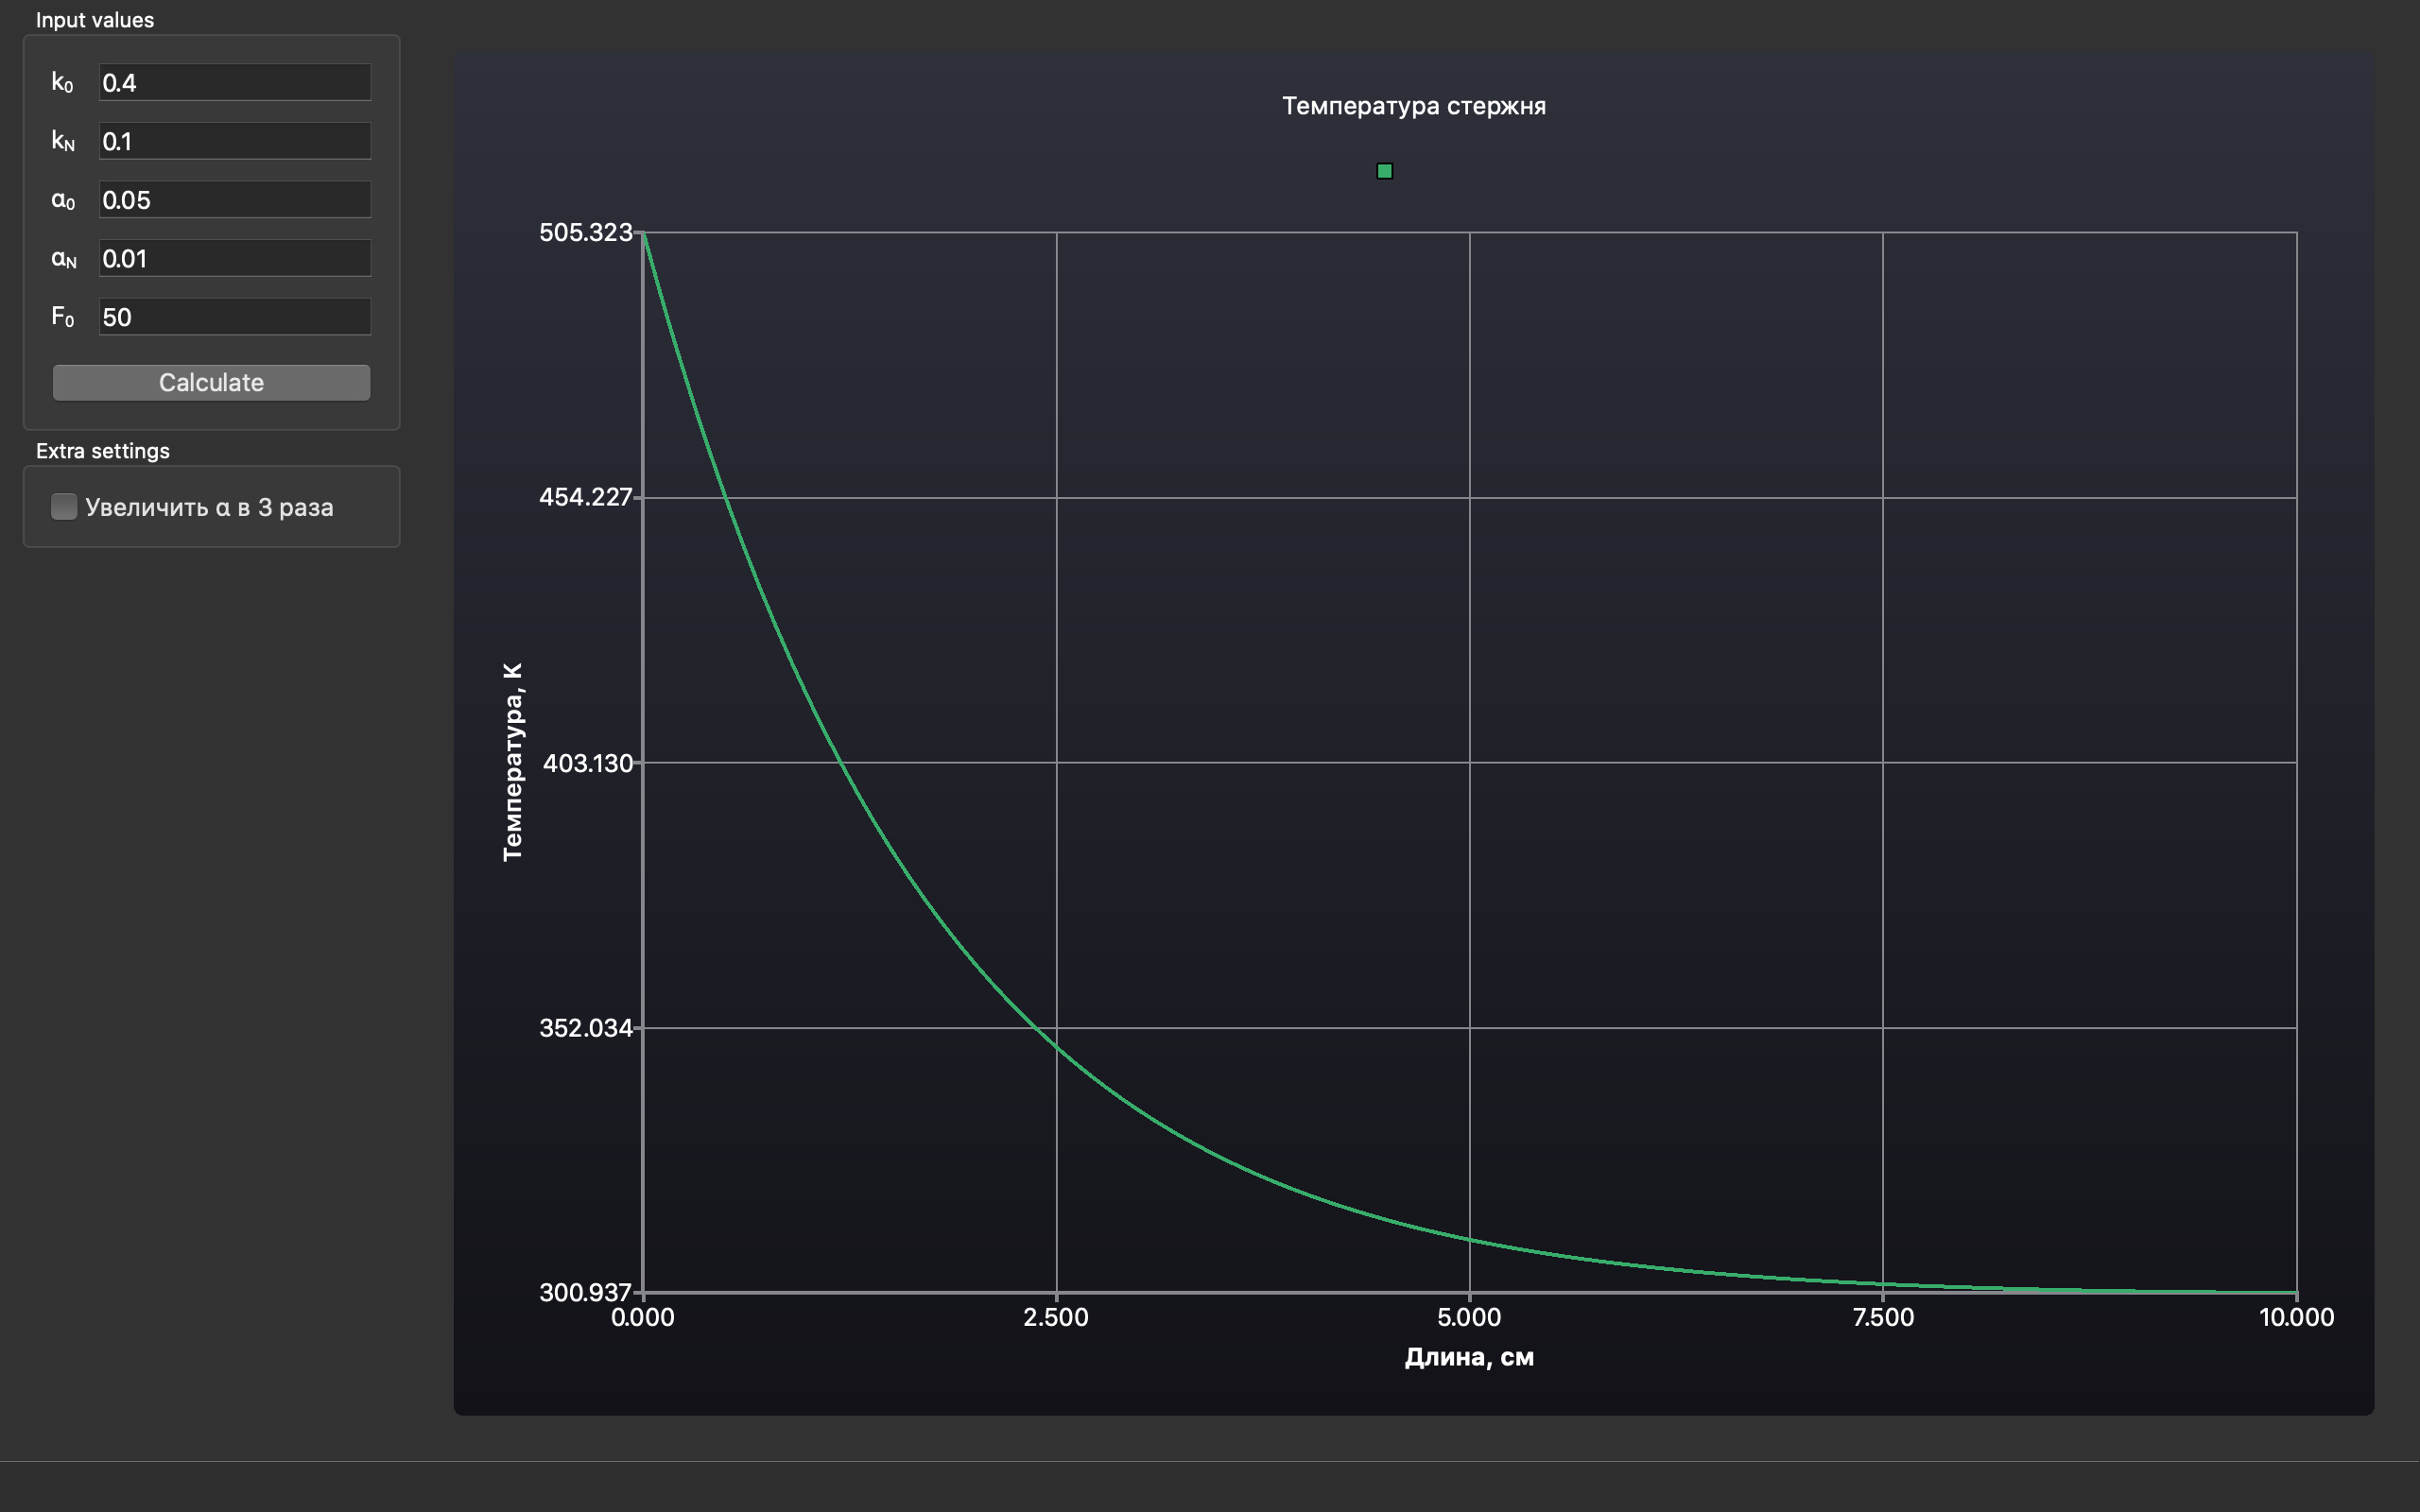
\includegraphics[scale=0.35]{img/Default.png}
    \caption{Исходные данные}
\end{figure}

\subsection{График при $F_0 = -10$}

\begin{figure}[H]
    \centering
    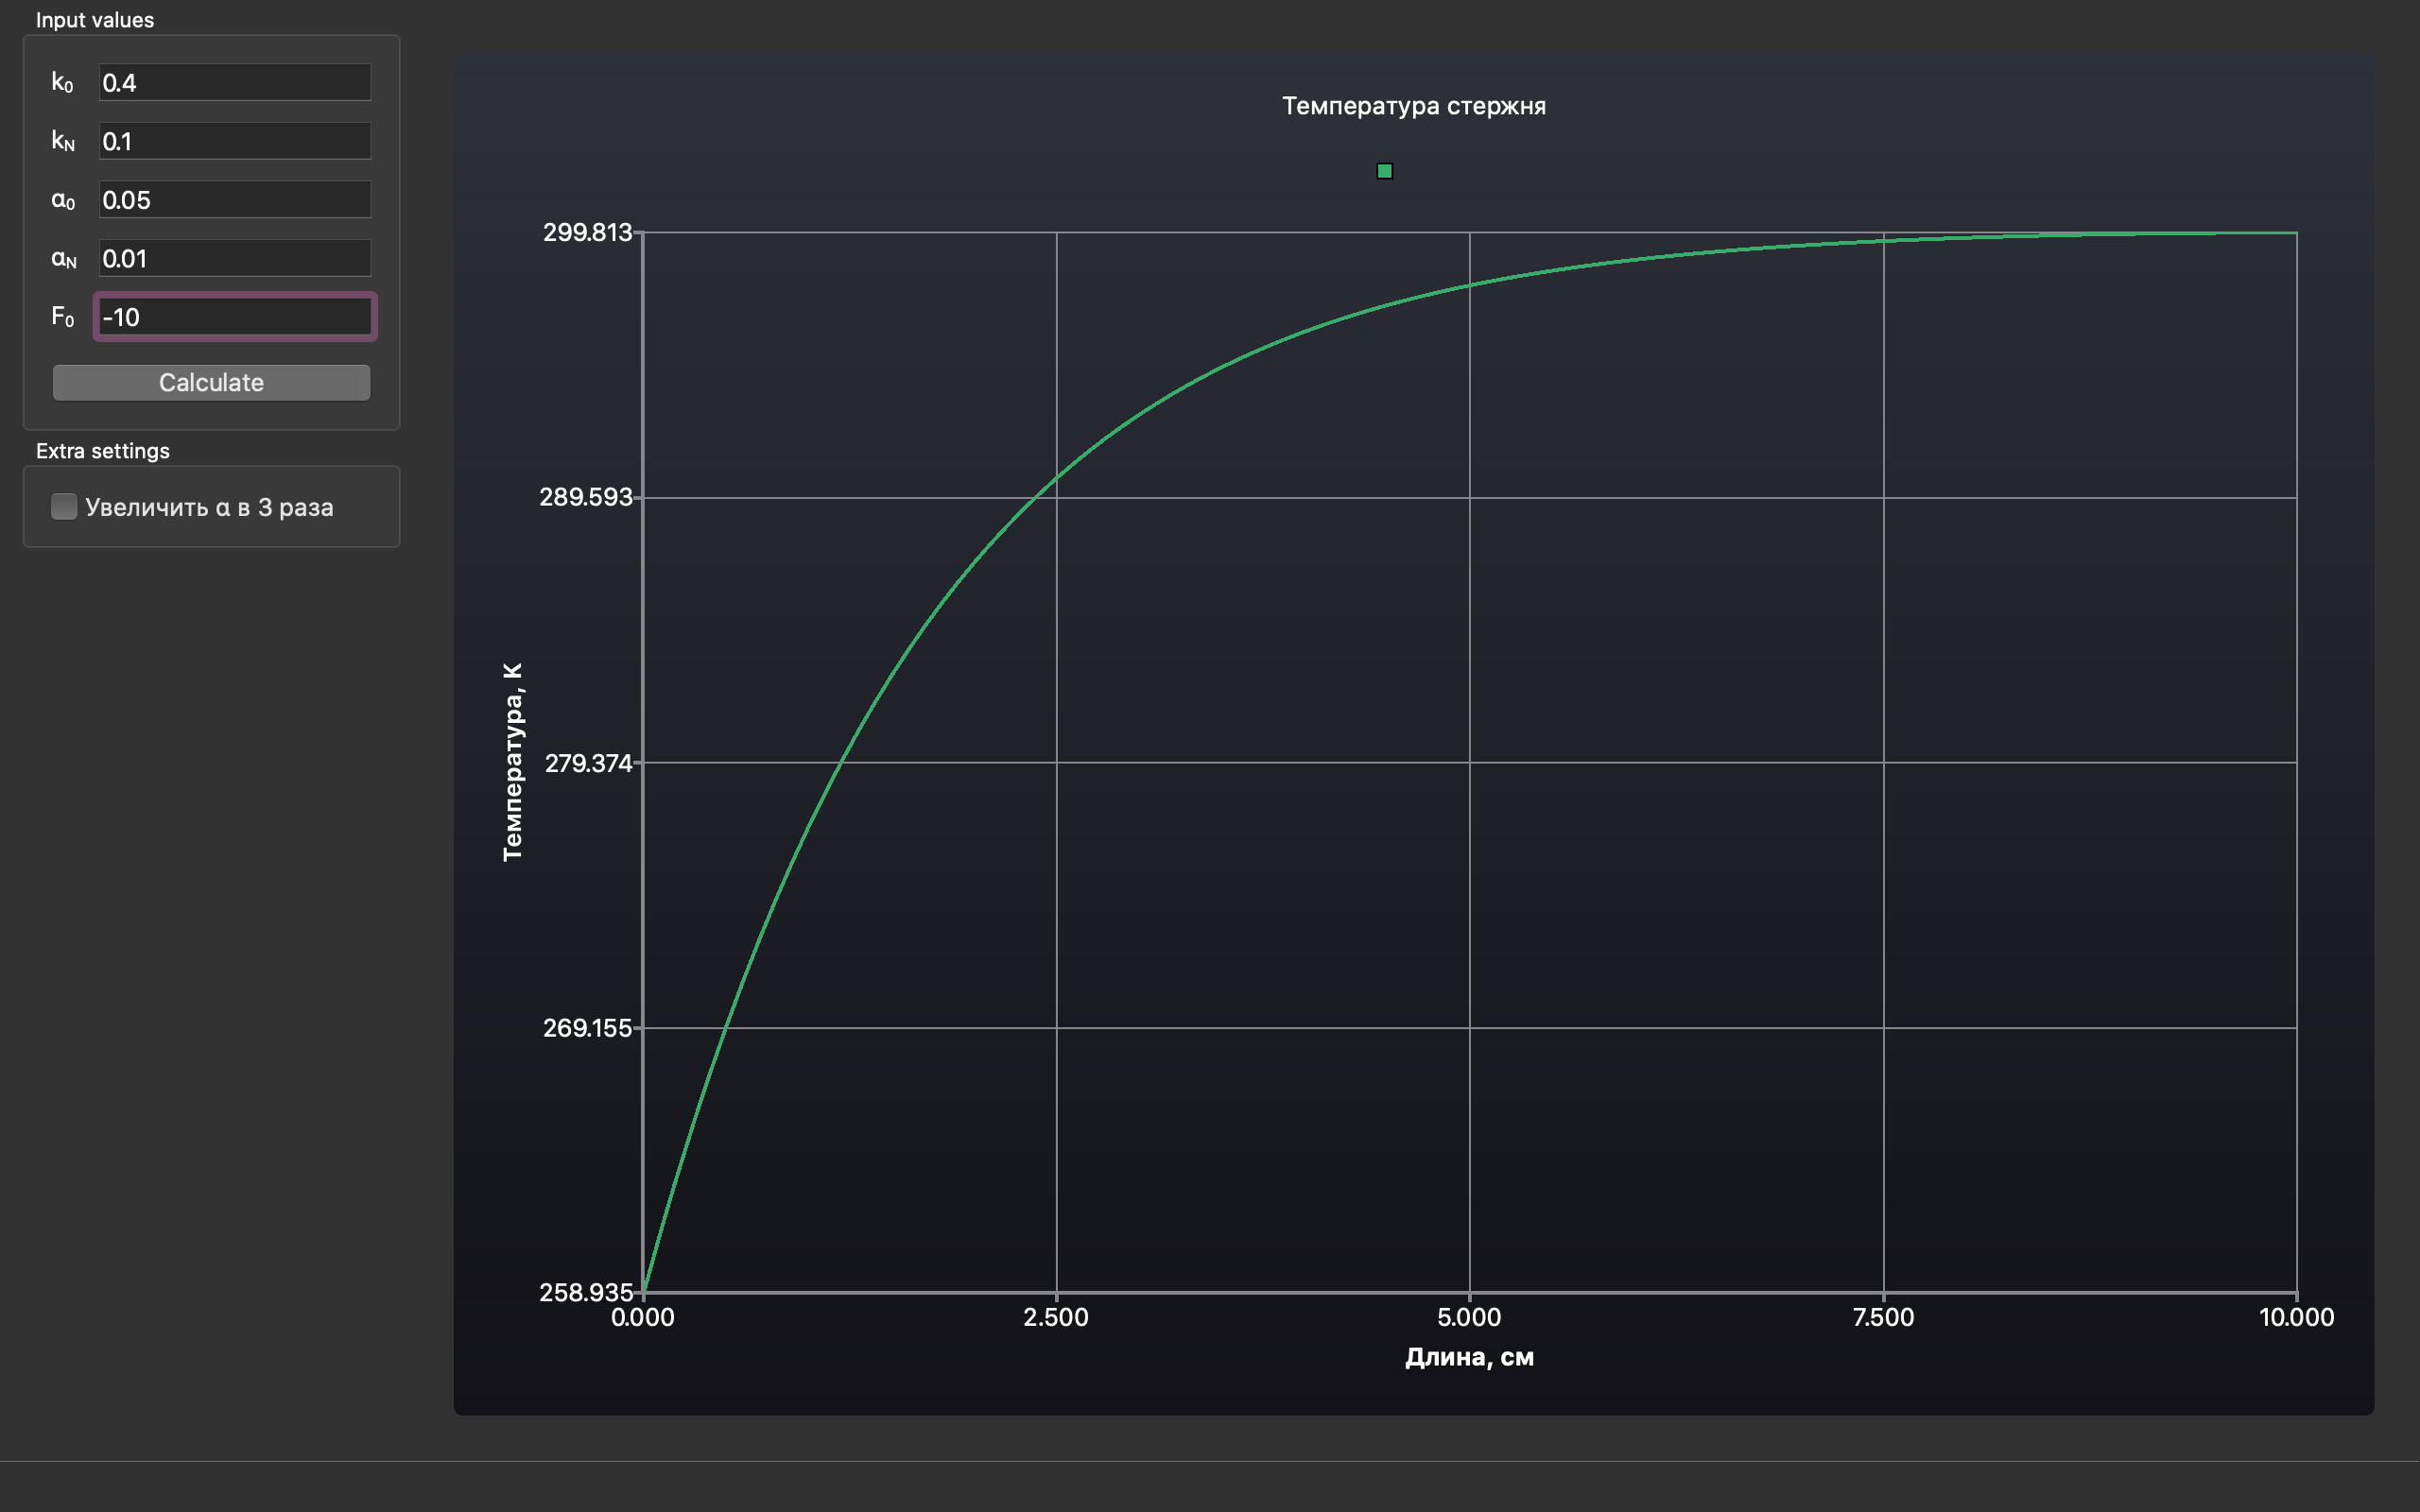
\includegraphics[scale=0.35]{img/LessZero.png}
    \caption{$F_0=-10$}
\end{figure}

\subsection{График при $\alpha$ увеличенное в 3 раза}

\begin{figure}[H]
    \centering
    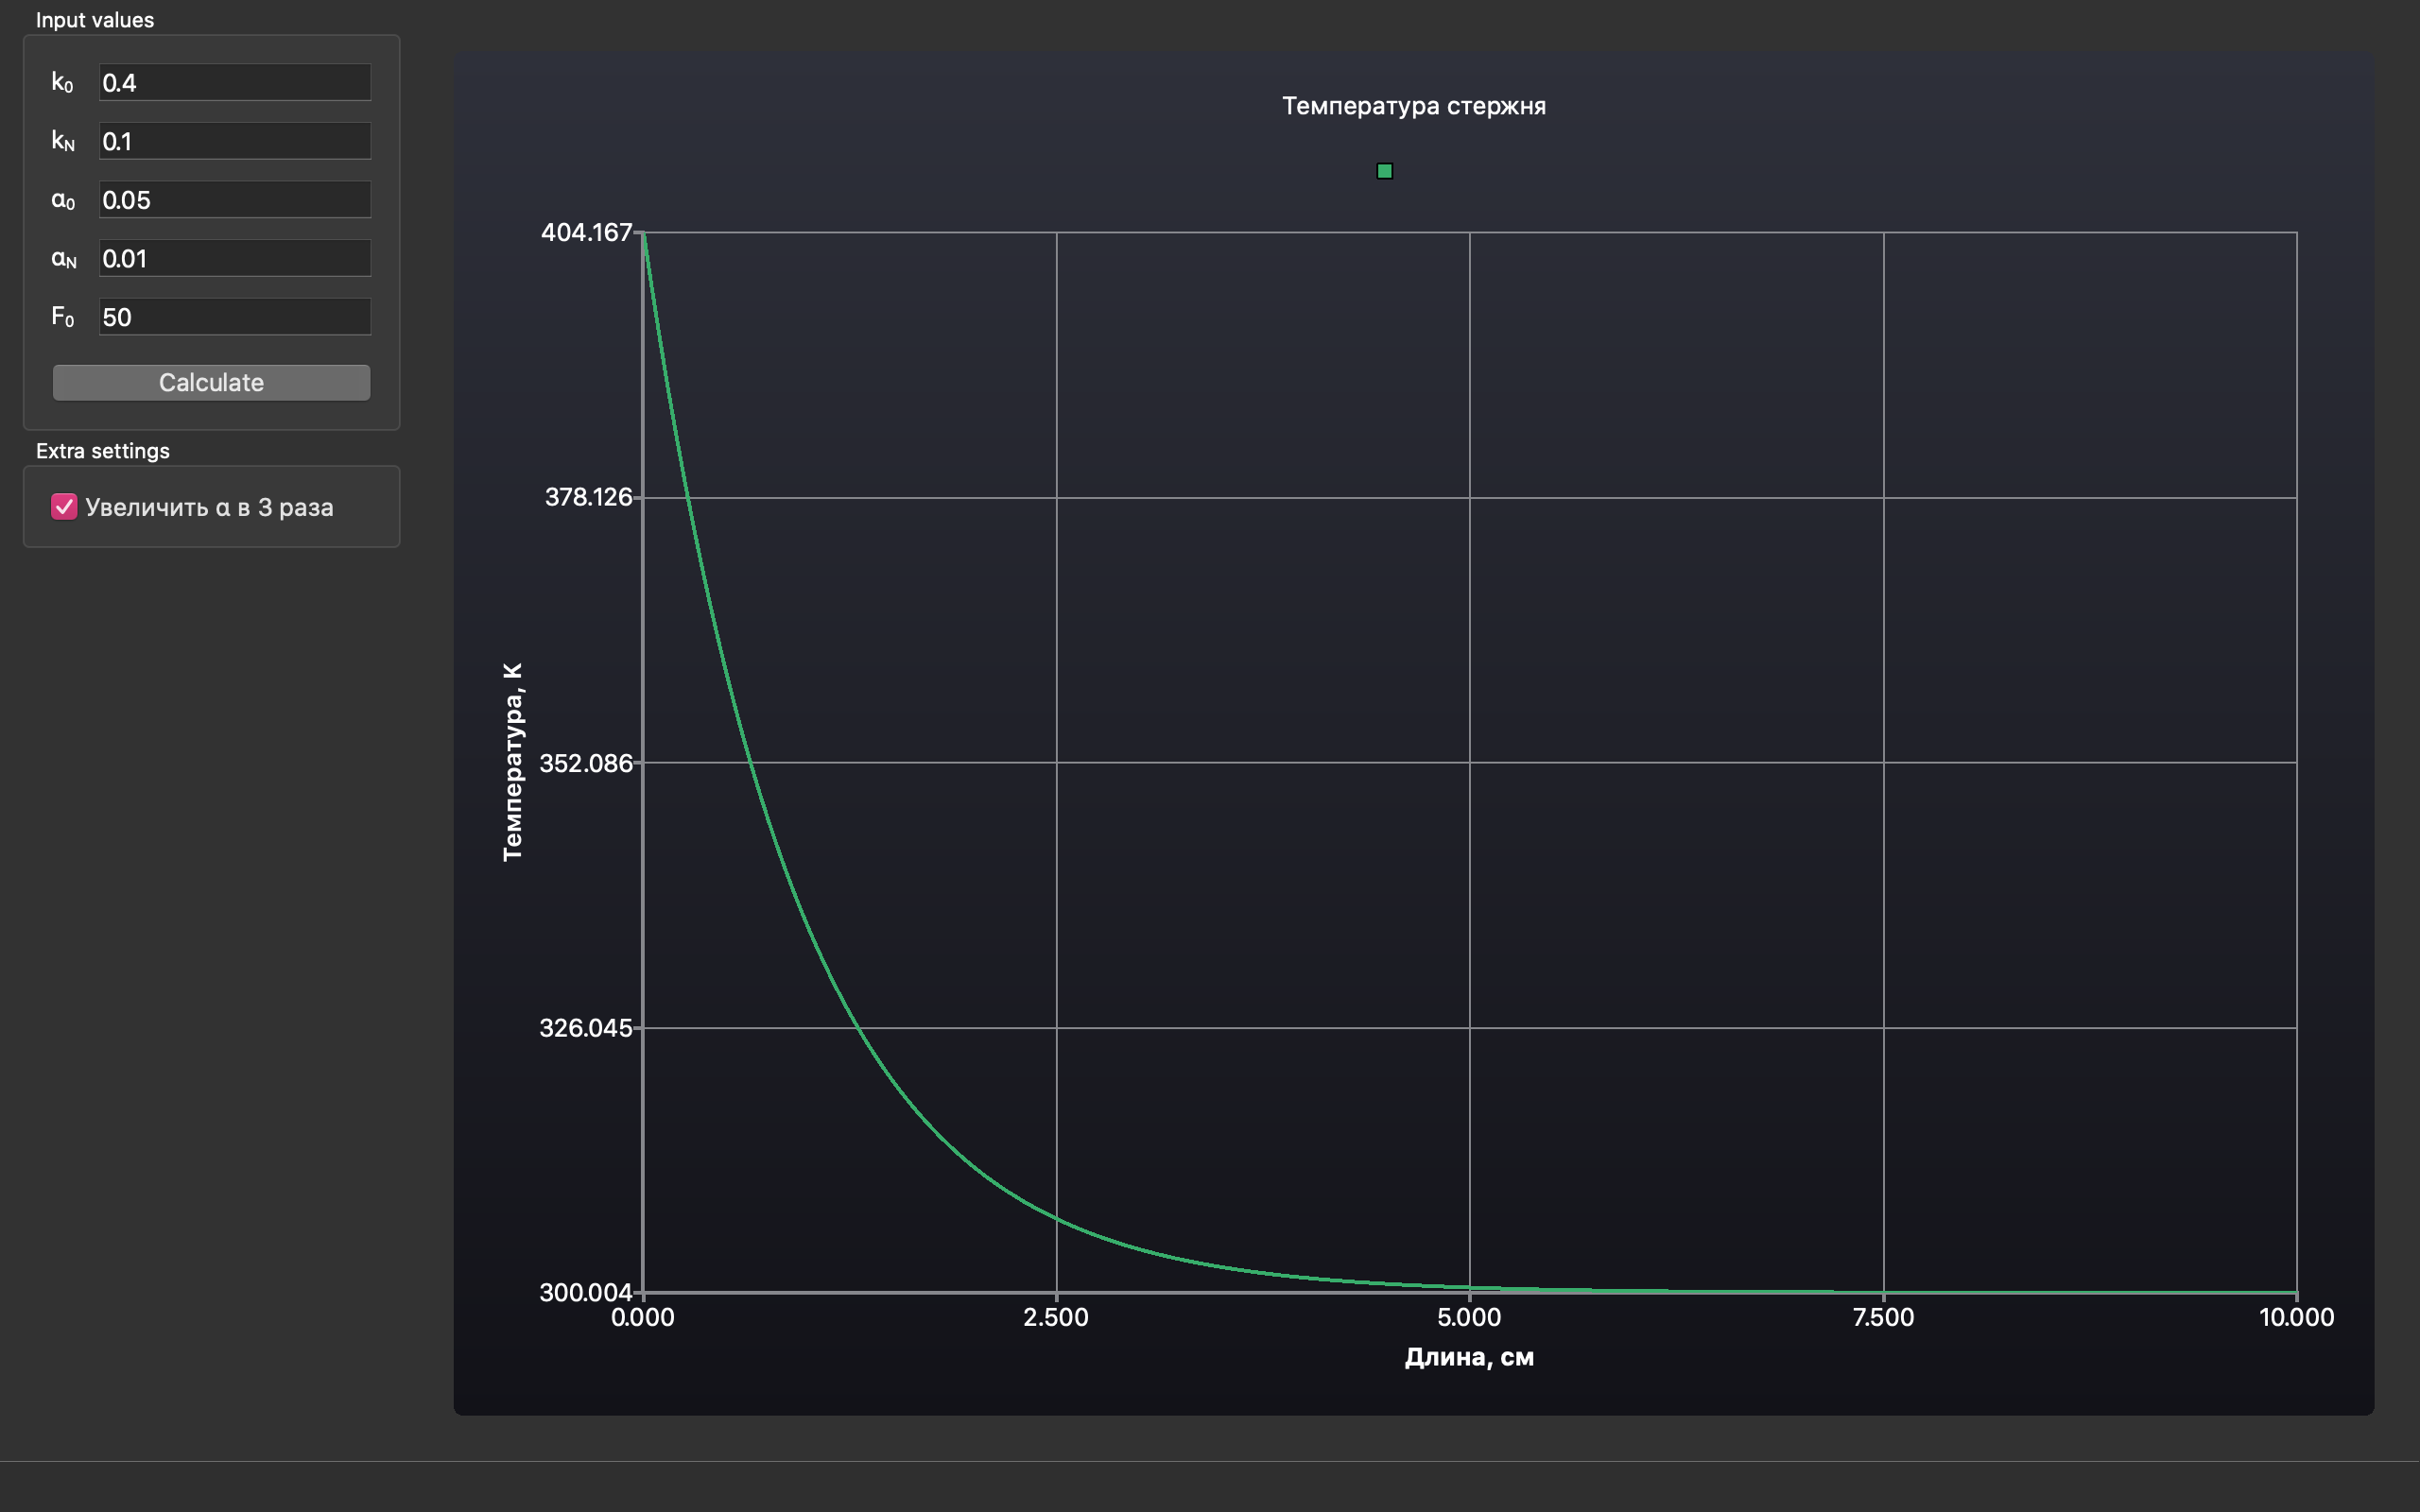
\includegraphics[scale=0.35]{img/AlphaX3.png}
    \caption{$\alpha$ увеличенное в 3 раза}
\end{figure}

\subsection{График при $F_0 = 0$}

\begin{figure}[H]
    \centering
    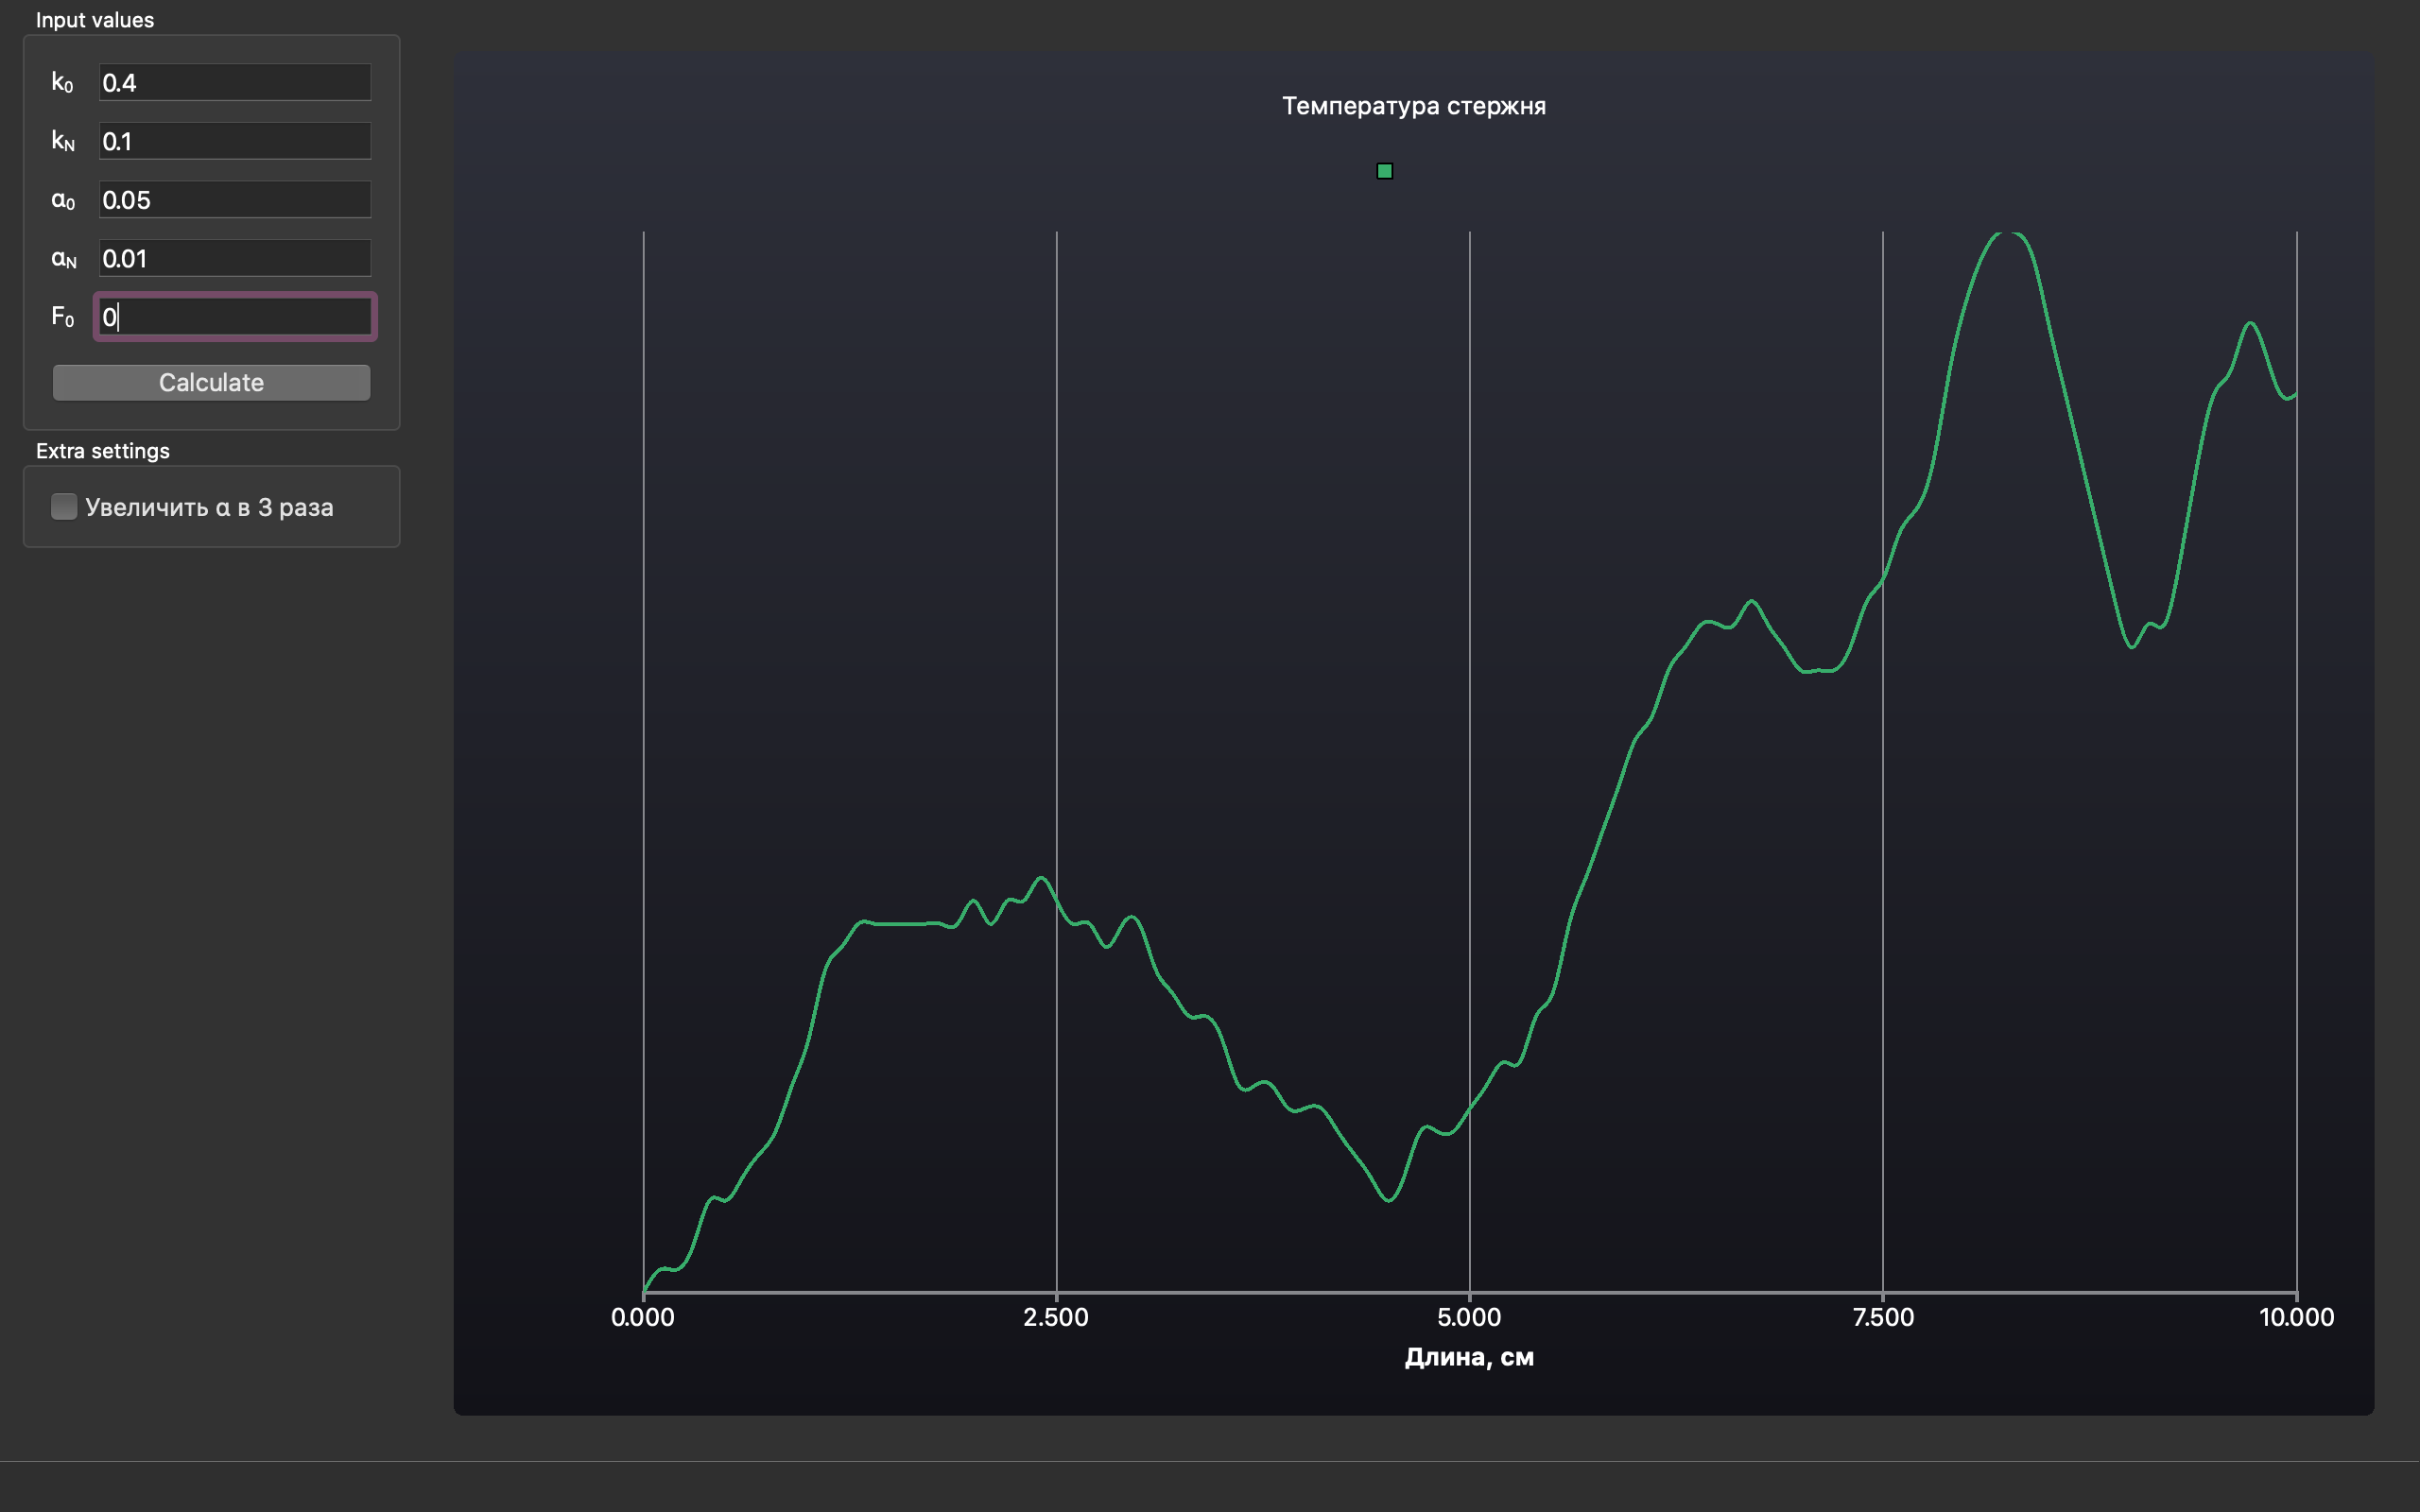
\includegraphics[scale=0.35]{img/Zero.png}
    \caption{$F_0 = 0$}
\end{figure}

Библиотека {\ttfamily QtCharts} приближает график по осям так, чтобы границы являлись максимальными и минимальными значениями графика, поэтому на этом графике не видно прямой. Выведем значения полученные программой и построим по ним график.

\begin{figure}[H]
    \centering
    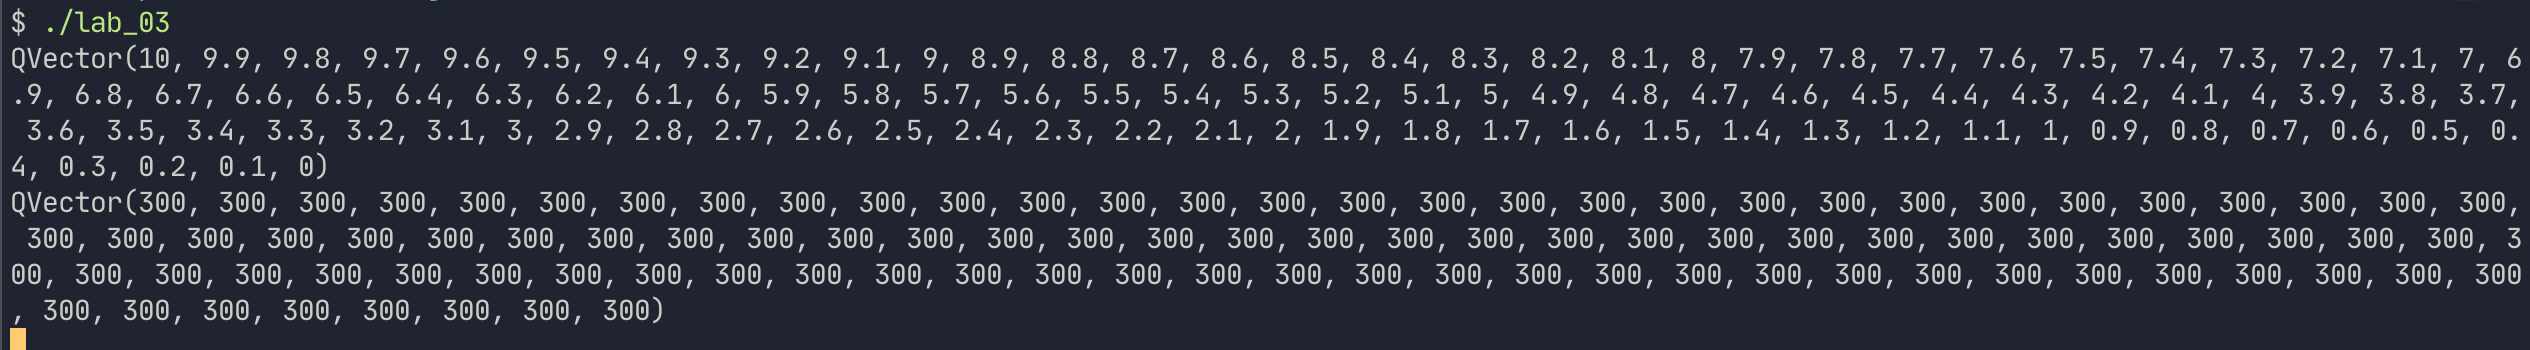
\includegraphics[scale=0.40]{img/ZeroPrint.png}
    \caption{Вывод программы}
\end{figure}

\begin{figure}[H]
    \begin{tikzpicture}
        \begin{axis}[
            legend pos = north west,
            xlabel=Длина стержня (см),
            ylabel=Температура (К),
            grid = major,
            width = 0.8\paperwidth,
            height = 0.38\paperheight,
            line width = 1
        ]
            \legend{
                Температура стержня
            };

            \addplot[black] coordinates {
                    (0.0, 300)
                    (1.0, 300)
                    (2.0, 300)
                    (3.0, 300)
                    (4.0, 300)
                    (5.0, 300)
                    (6.0, 300)
                    (7.0, 300)
                    (8.0, 300)
                    (9.0, 300)
                    (10.0, 300)
            };
        \end{axis}
    \end{tikzpicture}
    \caption{$F_0=0$}
    \label{img:noteven}
\end{figure}

\section{ВОПРОСЫ}

\subsection{Какие способы тестирования программы можно предложить?}

\begin{enumerate}
    \item Ввести $F_0$ (тепловой поток) меньше нуля. Это означает, что съем тепла идет слева, поэтому температура будет увеличиваться от $0$ до $l$.
    \item Ввести $F_0$ (тепловой поток) равным нулю. Это значит, что тепловое нагружение отсутствует, поэтому температура стержня будет везде равна температуре окружающей среды.
    \item Увеличить значения коэффициента теплоотдачи в несколько раз, Это значит, что стержень будет отдавать больше тепла и скорость снижения температуры будет увеличена.
\end{enumerate}

\subsection{Получите простейший аналог нелинейного краевого условия при $x = l$}

\begin{equation*}
    x = l, -k(l) \frac{dT}{dx} = \alpha_N \big( T(l) - T_0 \big) + \varphi(T)
\end{equation*}

, где $\varphi(T)$ -- заданная функция. Производную аппроксимируйте односторонней разностью.

Заменяем производную разностью

\begin{equation*}
    -k(l) \frac{T(x + h) - T(x)}{h} = \alpha_N \big( T(l) - T_0 \big) + \varphi(T)
\end{equation*}

При $x = l$ полуаем

\begin{equation*}
    -k(l) \frac{T(l) - T(l-1)}{h} = \alpha_N \big(T(l) - T_0 \big) +
    \varphi \big(T(l) \big)
\end{equation*}

Заменим $k(l) = k_l, T(l) = T_l$

\begin{equation*}
    k_l T_{l-1} - k_l T_l = \alpha_N T_l h - \alpha_NT_0 h + \varphi(T_l) h
\end{equation*}

\begin{equation*}
    \big( k_l + \alpha_N h \big) T_l - k_l T_{l-1} = \big( \alpha_NT_0 - \varphi(T_l) \big) h
\end{equation*}

\subsection{Опишите алгоритм применения метода прогонки, если при $x=0$ краевое условие линейное (как в настоящей работе), а при $x=l$, как в п.2}

\begin{equation*}
    \begin{cases}
        x = 0, -k(0) \frac{dT}{dx} = F_0 \\
        x = l, -k(l) \frac{dT}{dx} = \alpha_N\big(T(l) - T_0\big) + \varphi(T) \\
    \end{cases}
\end{equation*}

Поскольку краевое условие при $x=0$ линейное, то будем использовать правую прогонку.

\begin{equation*}
    y_n = \varepsilon_{n+1} y_{n+1} + \eta_{n+1}
\end{equation*}

Используем аппроксимацию первого порядка точности для краевого условия $x=0$

\begin{equation*}
    -k_0 \frac{T_1 - T_0}{h} = F_0
\end{equation*}

\begin{equation*}
    T_0 - T_1 = \frac{F_0h}{k_0}
\end{equation*}

\begin{equation*}
    \begin{cases}
        K_0 = 1 \\
        M_0 = -1 \\
        P_0 = \frac{F_0h}{k_0} \\
    \end{cases}
\end{equation*}

Разностная аппроксимация для краевого условия $x=l$ будет иметь вид

\begin{equation*}
    -k_l \frac{T_l - T_{l-1}}{h} = \alpha_N\big(T_l - T_0\big) + \varphi(T_l)
\end{equation*}

\begin{equation*}
    k_lT_{l-1} + k_lT_l = \alpha_N T_l h - \alpha_NT_0 h + \varphi(T_l) h
\end{equation*}

\begin{equation*}
    k_lT_{l-1} + (k_l - \alpha_Nh)T_l = \varphi(T_l)h - \alpha_NT_0h
\end{equation*}

\begin{equation*}
    \begin{cases}
        K_l = k_l - \alpha_Nh \\
        M_l = k_l \\
        P_l = \varphi(T_l)h - \alpha_NT_0h \\
    \end{cases}
\end{equation*}

Начальные прогоночные коэффициенты будут равны

\begin{equation*}
    \begin{cases}
        \varphi_1 = -\frac{M_0}{K_0} \\
        \eta_1 = \frac{P_0}{K_0}
    \end{cases}
\end{equation*}

Значение $T$ в точке $l$ будет равно

\begin{equation*}
    T_l = \frac{P_l - M_l \eta_l}{K_l + M_l \varepsilon_l}
\end{equation*}

\subsection{Опишите алгоритм определения единственного значения сеточной функции $y_p$ в одной заданной точке $p$. Использовать встречную прогонку, то есть комбинацию правой и левой прогонок. Краевые условия линейны.}

Метод встречных прогонок подразумевает, что на промежутке $0 \le n \le p + 1$ будет использоваться правая прогонка, а на промежутке $p \le n \le N$ -- левая.

Тогда коэффициенты для правой прогонки будут

\begin{equation*}
    \varepsilon_{n+1} = \frac{C_n}{B_n-A_n\varepsilon_n}
\end{equation*}

\begin{equation*}
    \eta_{n+1} = \frac{D_n + A_n \eta_n}{B_n - A_n \varepsilon_n}
\end{equation*}

\begin{equation*}
    0 \le n \le p+1
\end{equation*}

Для левой прогонки:

\begin{equation*}
    \xi_{n-1} = \frac{C_n}{B_n - A_n \xi_n}
\end{equation*}

\begin{equation*}
    \pi_{n-1} = \frac{A_n\pi_n + D_n}{B_n - A_n\xi_n}
\end{equation*}

\begin{equation*}
    p \le n \le N
\end{equation*}

Тогда

\begin{equation*}
    \begin{cases}
        y_n = \varepsilon_{n+1}y_{n+1}+\eta_{n+1} \\
        y_{n+1} = \xi_{n}y_{n} + \pi_{n} \\
    \end{cases}
\end{equation*}

Подставим вместо $n$ $p$, получим

\begin{equation*}
    \begin{cases}
        y_p = \varepsilon_{p+1}y_{p+1}+\eta_{p+1} \\
        y_{p+1} = \xi_{p}y_{p} + \pi_{p} \\
    \end{cases}
\end{equation*}

\begin{equation*}
    y_p = \varepsilon_{p+1}\xi_py_p + \varepsilon_{p+1}\pi_p + \eta_{p+1}
\end{equation*}

\begin{equation*}
    y_p = \frac{\varepsilon_{p+1}\pi_p + \eta_{p+1}}{1 - \varepsilon_{p+1}\xi_{p}}
\end{equation*}
